%%==============================================================
%% Autor: Matheus dos Reis de Jesus
%% Última versão Maio/2021
%% Arquivo em formato UTF-8
%% Compilar com pdftex
%% Precisa do arquivo abntex2-UFV.sty e abntex2cite.tex
%%
%% Modelo: Rodrigo Smarzaro (smarzaro@ufv.br)
%%==============================================================

\documentclass[
	% -- opções da classe memoir --
	12pt,				    % tamanho da fonte
	openright,			    % capítulos começam em pág ímpar (insere página vazia caso preciso)
	oneside,			    % para impressão só no anverso. Oposto a twoside
	a4paper,			    % tamanho do papel.
    % -- opções do pacote abntex2 --
    % chapter=TITLE,         % Títulos em maiúsculas
    sumario=tradicional,    % Sumário padrão memoir (mais bonito "imo")
    % -- opções do pacote babel --
	english,			    % idioma adicional para hifenização
	brazil,				    % o último idioma é o principal do documento
	]{abntex2}              % Personaliza a capa. Precisa do arquivo ufv.cls para funcionar.


% Pacotes fundamentais
\usepackage{abntex2-UFV}        % Personalização para a Universidade Federal de Viçosa
\usepackage{lmodern}			% Usa a fonte Latin Modern			
\usepackage[T1]{fontenc}		% Selecao de codigos de fonte de saída
\usepackage[utf8]{inputenc}		% Codificacao do documento (conversão automática dos acentos)
\usepackage{indentfirst}		% Indenta o primeiro parágrafo de cada seção.
\usepackage{graphicx}			% Inclusão de gráficos
\usepackage{float}				% Posicionamento específico de figuras
\usepackage{booktabs}           % \toprule, \midrule e \bottomrule para tabelas
\usepackage{hyperref}
% Sistema autor-data com títulos nas referências em negrito
\usepackage[alf,abnt-emphasize=bf]{abntex2cite}	

% ---
% CONFIGURAÇÕES DE PACOTES
% ---

% Informações de dados para CAPA e FOLHA DE ROSTO
\titulo{\emph{UI Framework em React Native acessível para idosos}}
\autor{Matheus dos Reis de Jesus}
\local{Viçosa}
\data{2021}
\orientador{Luciano Rodrigues Costa}    % redefinido no abntex2-UFV para aceitar Instituição (default = UFV-CRP)
%\coorientador{Nome do Coorientador}
\instituicao{Universidade Federal de Viçosa}

\campus{\emph{Campus} de Viçosa}      % pacote abntex2-UFV
\curso{Ciência da Computação}               % pacote abntex2-UFV
%\membrobancaA{Membro da Banca A}             % pacote abntex2-UFV default = UFV-CRP
%\membrobancaB[UFMG]{Membro da Banca B}       % pacote abntex2-UFV default = UFV-CRP
%\databanca{\today}                           % pacote abntex2-UFV

% O preambulo deve conter o tipo do trabalho, o objetivo,
% o nome da instituição e a área de concentração
\preambulo{Projeto apresentado à Universidade Federal de Viçosa como parte das exigências para a aprovação na disciplina de Metodologia de Pesquisa}
% ---

% ---
% Configurações de aparência do PDF final

% informações para o arquivo pdf de saída
% Interessante alterar a cor dos links para preto(black)
% para imprimir
\makeatletter
\hypersetup{
        % metadados
		pdftitle={\@title},
		pdfauthor={\@author},
    	pdfsubject={\imprimirpreambulo},
	    pdfcreator={LaTeX with abnTeX2},
		colorlinks=true,   % false: links em frame; true: links coloridos
    	linkcolor=black,    % cor dos links no documento
    	citecolor=blue,    % cor dos links para a bibliografia
    	filecolor=magenta, % cor dos links para arquivos
		urlcolor=blue,     % cor dos links para sites
		bookmarksdepth=4   % profundidade do sumário do PDF
}
\makeatother
% ---

\begin{document}
% Retira espaço extra obsoleto entre as frases.
\frenchspacing

% ----------------------------------------------------------
% ELEMENTOS PRÉ-TEXTUAIS
% ----------------------------------------------------------
\pretextual

% Capa
\imprimircapa

% Folha de rosto
\imprimirfolhaderosto
% ---

% Inserir folha de aprovação
%\imprimirfolhadeaprovacao

% Dedicatória
%\begin{dedicatoria}
%   \vspace*{\fill}
%   \centering
%   \noindent
%   \textit{Texto qualquer da dedicatória}
%   \vspace*{\fill}
%\end{dedicatoria}
% ---

% Agradecimentos
%\begin{agradecimentos}

%\end{agradecimentos}
% ---

% Epígrafe
%\begin{epigrafe}
%    \vspace*{\fill}
%	\begin{flushright}
%		\textit{``Word? nunca mais.''\\
%		(Qualquer usuário de \LaTeX)}
%	\end{flushright}
%\end{epigrafe}
% ---

% RESUMOS

% resumo em português
%\begin{resumo}
% \noindent
%Insira o resumo aqui

%\vspace{\onelineskip}

%\noindent
% \textbf{Palavras-chaves}: React Native, Framework, UI , Acessibilidade, UFV.
%\end{resumo}

% resumo em inglês
%\begin{resumo}[Abstract]
% \begin{otherlanguage*}{english}
%   \noindent
%   % Insira o abstract aqui
%
%   \vspace{\onelineskip}
%
%   \noindent
%   \textbf{Key-words}: TCC, latex, abntex, UFV..
% \end{otherlanguage*}
%\end{resumo}

% inserir lista de ilustrações
%\pdfbookmark[0]{\listfigurename}{lof}
%\listoffigures*
%\cleardoublepage
% ---

% inserir lista de tabelas
%\pdfbookmark[0]{\listtablename}{lot}
%\listoftables*
%\cleardoublepage
% ---


% inserir o sumario
\pdfbookmark[0]{\contentsname}{toc}
\tableofcontents*
\cleardoublepage
% ---

% ----------------------------------------------------------
% ELEMENTOS TEXTUAIS
% ----------------------------------------------------------
\textual

\chapter{Introdução}\label{sec:introducao}

Segundo a \emph{30ª Pesquisa Anual de Uso de TI},
realizada pela \emph{Fundação Getúlio Vargas}\cite{pesquisati30}, em abril de 2019 o Brasil já contava com aproximadamente 230 milhões de dispositivos móveis, pouco mais de 1 dispositivo móvel por habitante. Já na 31ª edição\cite{pesquisati31}, de junho de 2020, esse valor passou para de 342 milhões de dispositivos móveis, equivalente a aproximadamente 1,6 dispositivos por habitante. De acordo com dados do sensos realizados pelo IBGE, a população idosa(pessoas adultas acima de 65 anos) no Brasil cresceu de 8.9 milhões em 2017 para 9.8 milhões em 2020, um aumento de aproximadamente 11\% em 3 anos\cite{ibge}.

\par

Com o crescimento vertiginoso do uso de dispositivos móveis, há um aumento da demanda por aplicações que possam atender às mais diversas necessidades das pessoas que os utilizam. Levando em consideração os dados citados previamente, é plausível considerar que boa parte dos novos dispositivos pertençam à pessoas da terceira idade, que comumente apresentam dificuldade para executar diversas ações que são essenciais na interação de dispositivos móveis, em especial, os com tela tátil. Além dos fatores mais comuns, pessoas idosas apresentam problemas motores, de visão e cognitivos, que tornam ainda mais difíceis essas interações. Segundo Claudia Zapata \emph{et al}, “O desenvolvimento de aplicações para dispositivo móveis se tornou uma forma de melhorar a qualidade de vida para idosos, já que é possível aplicar a vários setores como a medicina, por exemplo”\cite{elderlyMainChallenges}.

\par

Este projeto foi idealizado a partir de um trabalho anterior: \textit{Um framework para facilitar as interações entre dispositivos móveis e pessoas idosas}\cite{tesedamaris}. Em sua tese, Dâmaris buscou identificar as ações em dispositivos móveis que os idosos enfrentam maior dificuldade para executar. Para conseguir identificar algumas dessas dificuldades, foram realizados testes em um trabalho conjunto com o \emph{Programa da Terceira Idade}, um projeto da Prefeitura Municipal de Viçosa - MG. Através destes testes foram identificadas algumas das ações que os idosos mais apresentam dificuldade em executar: o movimento de pinça, movimento de rotação e digitação.

\par

Com o resultado das pesquisas em mãos, foi então criado o \textit{ElderlyFrame}\cite{elderlyframe}, um \textit{framework} de interface de usuário nativo para \textit{Android}. O projeto contém um conjunto de componentes visuais com o objetivo de facilitar ações que geralmente exigem mais coordenação motora e acuidade visual. A seguir, temos os exemplos destes componentes que foram implementados.

\begin{figure}[H]
	\begin{center}
		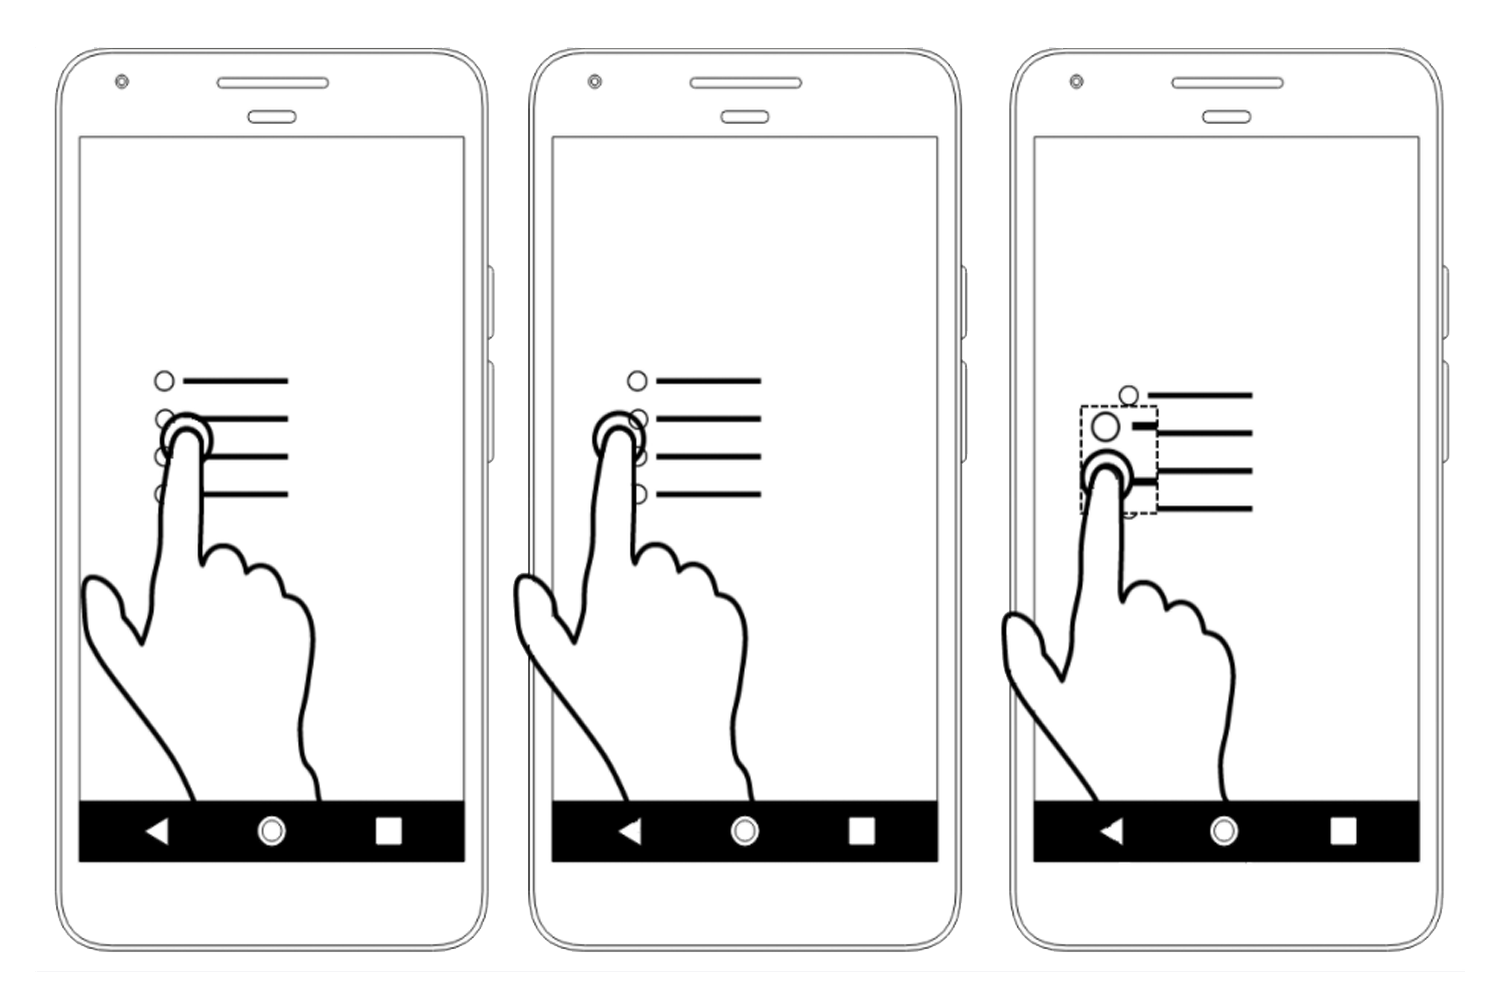
\includegraphics[height=0.4\linewidth]{touchable-zoom.png}
	\end{center}
	\caption[Touchable Zoom]{Componente de Zoom por toque do \textit{ElderlyFrame}}
	\label{fig:touchableZoom}
\end{figure}

\begin{figure}[H]
	\begin{center}
		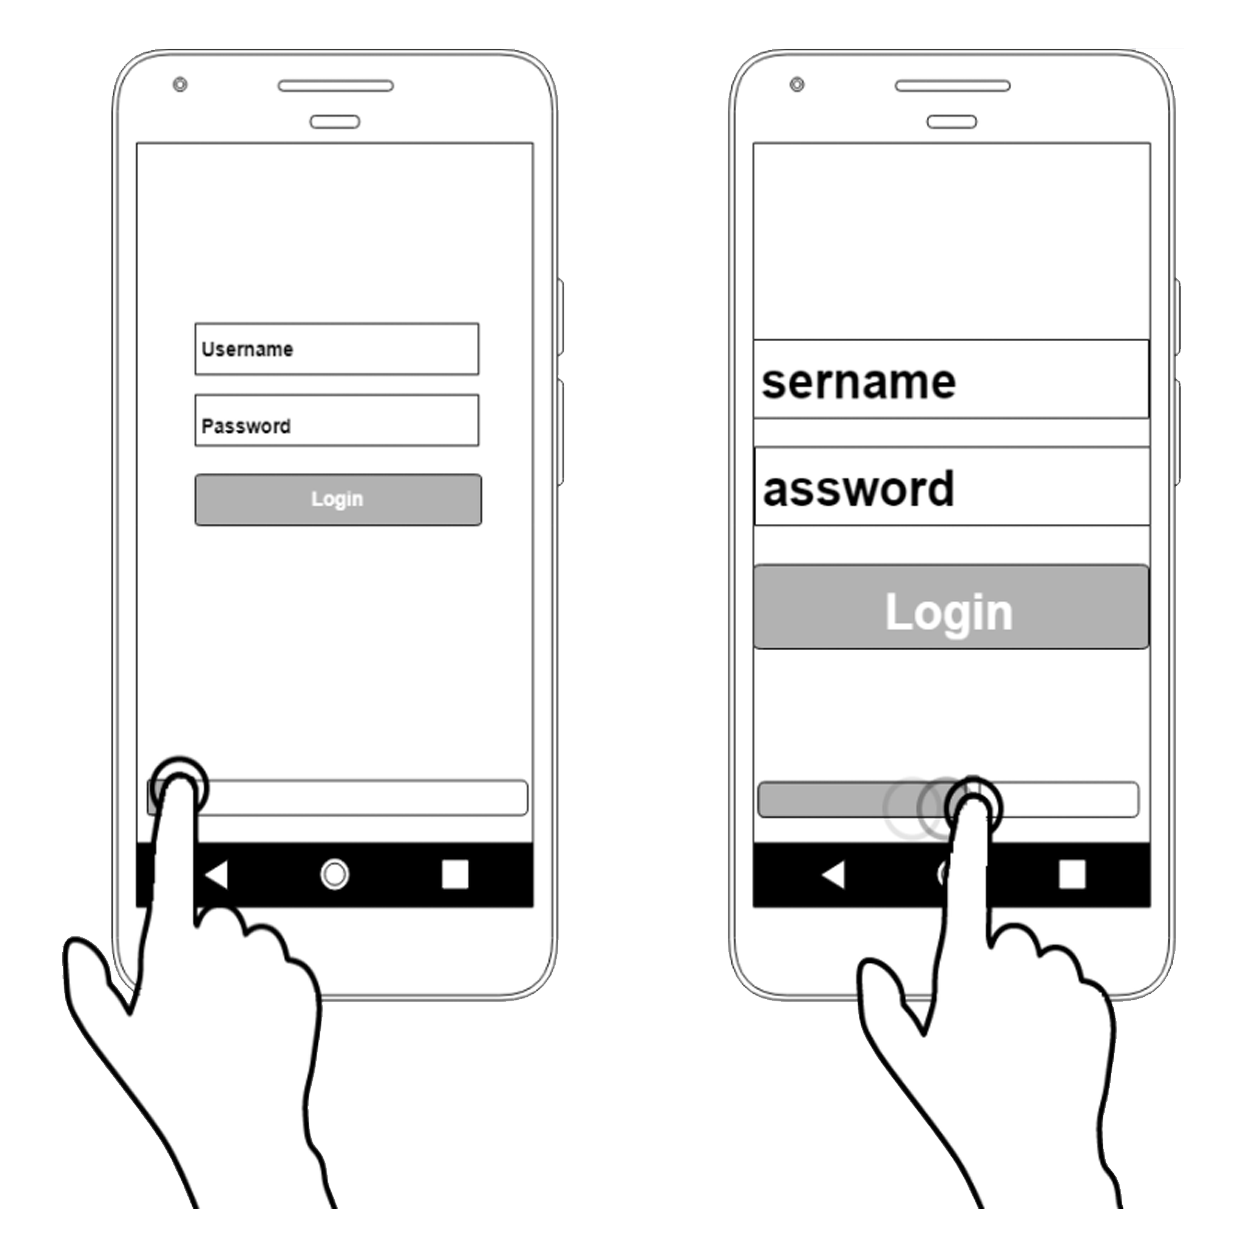
\includegraphics[height=0.5\linewidth]{zoom-bar.png}
	\end{center}
	\caption[Componente de zoom com barra]{Componente de Zoom por barra do \textit{ElderlyFrame}}
	\label{fig:zoomBar}
\end{figure}

\begin{figure}[H]
	\begin{center}
		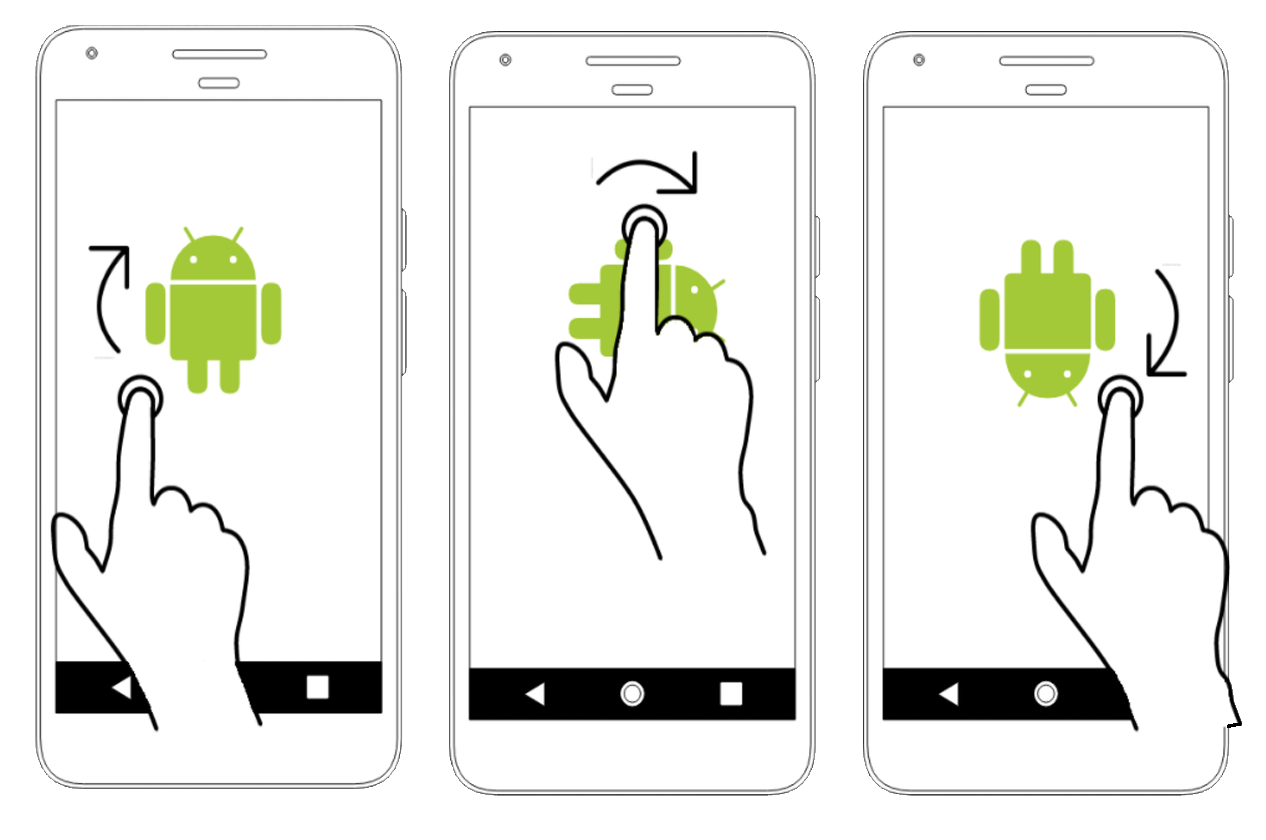
\includegraphics[height=0.5\linewidth]{rotation.png}
	\end{center}
	\caption[Componente de Rotação com apenas um dedo]{Componente de rotação com apenas um dedo do \textit{ElderlyFrame}}
	\label{fig:rotation}
\end{figure}

\begin{figure}[H]
	\begin{center}
		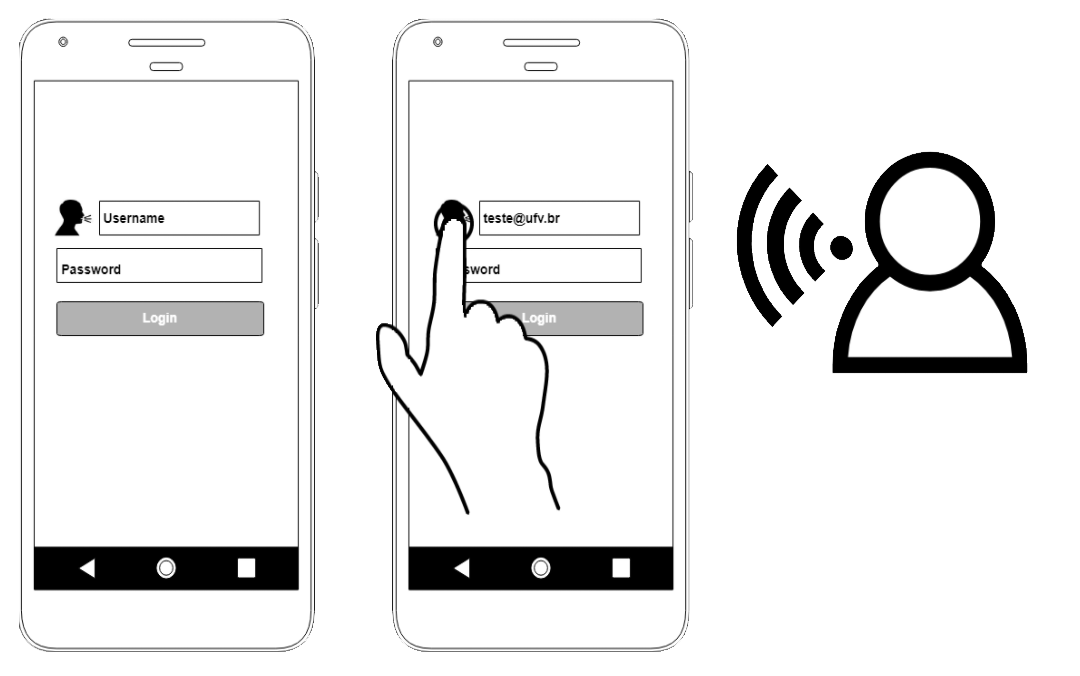
\includegraphics[height=0.5\linewidth]{speech-to-text.png}
	\end{center}
	\caption[Speech To Text]{Componente de conversão de voz para texto (\textit{speech-to-text}) do \textit{ElderlyFrame}}
	\label{fig:speechToText}
\end{figure}

\chapter{Justificativa}\label{sec:justificativa}

Atualmente existe implementações para \textit{React Native} de ferramentas que facilitam a presença de recursos de acessibilidade em aplicações para dispositivos móveis. Porém, estas ferramentas utilizam apenas recursos já existentes, funcionando apenas como facilitadoras. Este é um diferencial do \textit{ElderlyFrame}, e consequentemente deste projeto, que traz uma nova abordagem para interações que pessoas idosas apresentam dificuldade em executar.

\par

Em pesquisas realizadas para elaboração deste projeto, somente foram encontrados artigos e teses que abordavam a teoria da acessibilidade para idosos. Conteúdos que abordavam a falta de inclusão digital da terceira idade,  a falta de recursos de acessibilidade em aplicações para dispositivos móveis e afins. Porém, foi notada uma carência de projetos que de fato produzissem algo para mudar este cenário. O \textit{ElderlyFrame} foi construído com este propósito, e essa também é uma das motivações desta pesquisa.

\par

Como dito anteriormente, o \textit{ElderlyFrame} é um \textit{framework} de interface de usuário nativo para \textit{Android}, e este é um fator limitante da sua utilização. Ampliar o impacto do projeto e abranger uma maior parcela do cenário de desenvolvimento para dispositivos móveis são fatores motivadores para este projeto. Para isto, decidiu-se por focar em uma tecnologia de desenvolvimento multiplataforma. Tecnologias de desenvolvimento multiplataforma permitem o desenvolvimento de aplicações para diferentes ambientes, como \emph{Android} e \emph{iOS}, utilizando uma mesma base de código. A tecnologia escolhida para análise nesta pesquisa foi \textit{React Native}, pois é utilizado em aplicações com grande representatividade, como \textit{Instagram}, \textit{AirBnb} e \textit{Uber}.

\begin{figure}[H]
	\begin{center}
		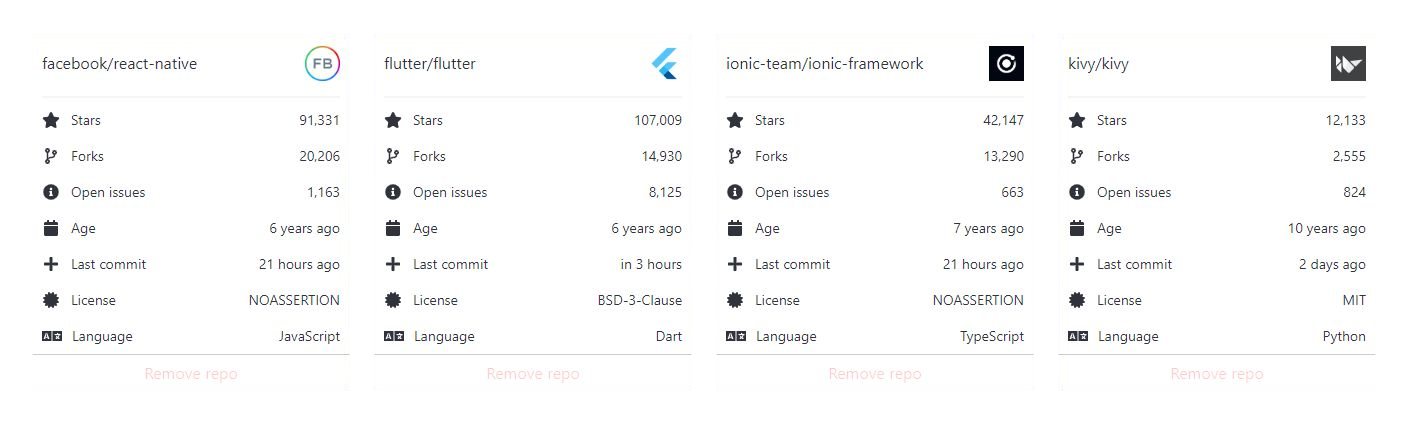
\includegraphics[width=1\linewidth]{github-compare.png}
	\end{center}
	\caption[GitHub Compare]{Comparação entre as estatísticas dos repositórios de tecnologias de desenvolvimento híbrido: \textit{React Native}, \textit{Flutter}, \textit{Ionic} e \textit{Kivy}}
	\label{fig:githubCompare}
	\legend{Fonte: \textit{GitHub Compare}. Disponível em \url{https://www.githubcompare.com/facebook/react-native+flutter/flutter+ionic-team/ionic-framework+kivy/kivy/}}
\end{figure}

A imagem acima mostra que o repositório do \textit{React Native}, no \textit{GitHub}, tem a maior quantidade de \textit{forks} e o 2º maior número de \textit{stars} e \textit{issues}, quando comparado com outras tecnologias de desenvolvimento multiplataforma, a saber: \textit{Flutter},\textit{Ionic} e \textit{Kivy}.

Além das estatísticas apresentadas no parágrafo anterior, foi usada como uma base uma pesquisa realizada pela \textit{Statista}, que aborda o uso de \textit{frameworks} para desenvolvimento multiplataforma. Como pode ser observado, o \textit{React Native} representa aproximadamente 42\% do uso em aplicações. Em um cenário com tantas opções, 42\% é um valor significativamente grande e que poderia ampliar o impacto dos resultados deste projeto.

\begin{figure}[H]
	\begin{center}
		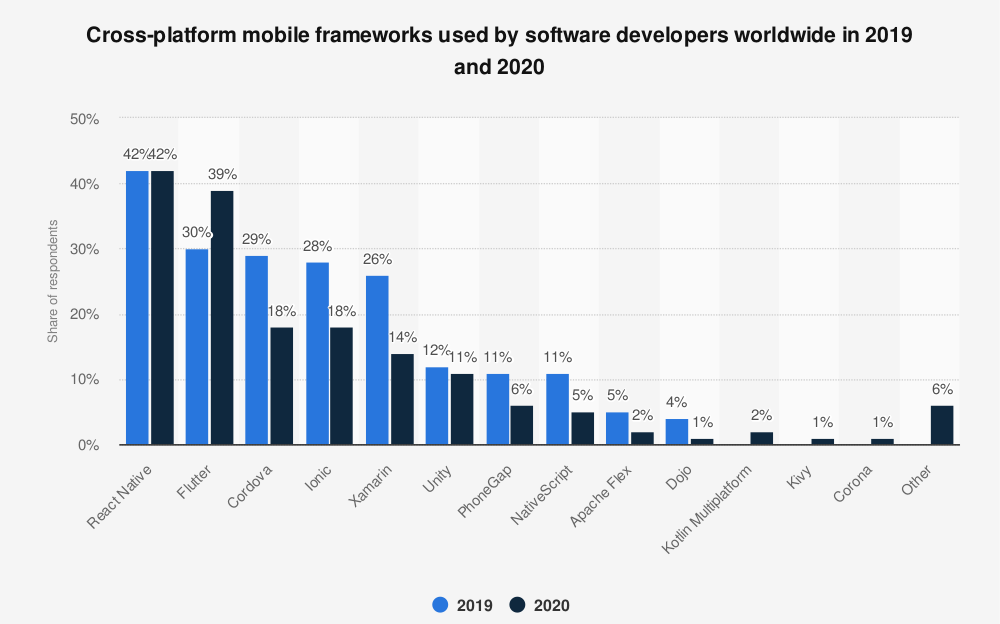
\includegraphics[height=.5\linewidth]{mobile-frameworks-statista.png}
	\end{center}
	\caption[GitHub Compare]{Comparação entre as estatísticas de uso de \textit{frameworks} para desenvolvimento multiplataforma}
	\label{fig:statistaResearch}
	\legend{Fonte: \textit{Statista}. Disponível em
		\url{https://www.statista.com/statistics/869224/worldwide-software-developer-working-hours/}}
\end{figure}

\chapter{Objetivo}\label{sec:objetivos}

\section{Geral}

A proposta deste trabalho é analisar a viabilidade de implementação do \emph{ElderlyFrame} utilizando \emph{React Native}, uma tecnologia para desenvolvimento híbrido para dispositivos móveis.

\section{Específicos}

Além da análise de viabilidade serão verificados os pontos em que o \emph{React Native} pode não ser suficiente para suprir as necessidades de implementação da ferramenta. A busca por novos recursos para serem adicionados ao escopo também será abordada, para complementar o trabalho.

\par

De acordo com Khan Kallimulah et al, "A tecnologia no campo da saúde deu um passo à frente para facilitar a manutenção da saúde no dia a dia"\cite{KALIMULLAH2017352}. Para ir além da análise conceitual, considera-se, para esse projeto, a criação de uma prova de conceito para validar se as implementações da ferramenta de fato atendem às necessidades mais comuns de pessoas idosas.

\chapter{Metodologia}\label{sec:metodologia}


Para análise da viabilidade do projeto foi escolhido o método de revisão bibliográfica. Buscar por fontes que validem ou contradigam a ideia desta pesquisa é essencial para refinamento de ideias. Encontrar trabalhos anteriores e em processo também se faz necessário, não apenas para validar a ideia, como também para ampliar a visão sobre a ferramenta e seu impacto.

\chapter{Cronograma}\label{sec:cronograma}

Para execução deste projeto, foram estabelecidas as atividades a serem realizadas e os meses que em que irão ocorrer durante o período deste projeto. O quadro a seguir apresenta essa relação:

\par

\begin{table}[htbp]
	\centering
	\caption[Cronograma mensal]{Cronograma do Projeto em Meses}
	\label{tab:cronogramaMensal}
	\begin{tabular}{lcccccccc} %|c|c|c|c|c|c|c|c|c|c|c|c
		\toprule
		\textbf{Atividade}    & \textbf{Fev} & \textbf{Mar} & \textbf{Abr} & \textbf{Mai} & \textbf{Jul} & \textbf{Ago} & \textbf{Set} & \textbf{Out} \\
		\midrule
		Análise do Tema       & $\bullet$    & $\bullet$    & $\bullet$    &              &              &              &              &              \\
		Revisão Bibliográfica &              & $\bullet$    & $\bullet$    & $\bullet$    & $\bullet$    &              &              &              \\
		Redação do Projeto    &              &              & $\bullet$    & $\bullet$    & $\bullet$    & $\bullet$    & $\bullet$    & $\bullet$    \\
		Implementação         &              &              &              & $\bullet$    & $\bullet$    & $\bullet$    &              &              \\
		Prova de Conceito     &              &              &              &              & $\bullet$    & $\bullet$    & $\bullet$    &              \\
		Validação da POC      &              &              &              &              &              & $\bullet$    & $\bullet$    & $\bullet$    \\
		\bottomrule
	\end{tabular}
	\fonte{Próprio Autor}
\end{table}


% As demandas de tempo(em horas) estimadas para orientação, desenvolvimento e revisão da literatura, do projeto escrito e demais artefatos produzidos são:

% \par

% \begin{table}[htpb]
% 	\centering
% 	\caption[Cronograma em horas]{Estimativa de tempo para cada atividade}
% 	\label{tab:cronogramaHoras}
% 	\begin{tabular}{lcc}
% 		\toprule
% 		\textbf{Item} & \textbf{Custeio} & \textbf{Tempo(horas)} \\
% 		\midrule
% 		Orientação    & Governo Federal  & 40                    \\
% 		Projeto       & Próprio          & 60                    \\
% 		Revisão       & Próprio          & 20                    \\
% 		\bottomrule
% 		Total         &                  & 120
% 	\end{tabular}
% 	\fonte{Próprio autor}
% \end{table}

% \chapter{Orçamento}\label{sec:orcamento}

% Estão orçados para este projeto os itens contidos na tabela abaixo, acompanhados de seus respectivos financiadores e valores:

% \par

% \begin{table}[htpb]
% 	\centering
% 	\caption[Orçamento]{Orçamento financeiro}
% 	\label{tab:orcamento}
% 	\begin{tabular}{lccc}
% 		\toprule
% 		\textbf{Item}                         & \textbf{Custeio} & \textbf{Custo} \\
% 		\midrule
% 		Computador Pessoal                    & Próprio          & R\$ 5000       \\
% 		Conexão com a \textit{Internet}       & Próprio          & R\$ 900        \\
% 		Licença para publicação na Play Store & Próprio          & ~R\$140        \\
% 		\bottomrule
% 		Total                                 &                  & R\$6040        \\
% 	\end{tabular}%
% 	\fonte{Próprio Autor}
% \end{table}%

% \chapter{Resultados Esperados}\label{sec:resultEsperados}

% ----------------------------------------------------------
% ELEMENTOS PÓS-TEXTUAIS
% ----------------------------------------------------------
\postextual

% Referências bibliográficas

%\bibliographystyle{abbrv}
\bibliography{referencias}

% Caso sejam necessários apêndices ou anexos em seu documento
% Use os ambientes abaixo

%% Apêndices
%
%% Inicia os apêndices
%\begin{apendicesenv}
%
%% Imprime uma página indicando o início dos apêndices
%\partapendices
%
%\chapter{Primeiro Apêndice}
%
%\chapter{Segundo Apêndice}
%
%\end{apendicesenv}
%
%
%% ----------------------------------------------------------
%% Anexos
%% ----------------------------------------------------------
%\begin{anexosenv}
%
%% Imprime uma página indicando o início dos anexos
%\partanexos
%
%\chapter{Primeiro Anexo}
%\lipsum[30]
%
%\chapter{Segundo Anexo}
%\lipsum[31]
%
%\end{anexosenv}

\end{document}